
\documentclass[12pt]{beamer}
\usepackage{amsmath}
\usepackage{mathtools}
\usepackage{multimedia}
\usepackage{hyperref}


\usefonttheme{professionalfonts} % using non standard fonts for beamer
\usefonttheme{serif} % default family is serif
%\documentclass[12pt]{beamerthemeSam.sty}
\usepackage{epsf}
%\usepackage{pstricks}
%\usepackage[orientation=portrait,size=A4]{beamerposter}
\geometry{paperwidth=160mm,paperheight=120mm}
%DT favorite definitions
\def\LL{\left\langle}	% left angle bracket
\def\RR{\right\rangle}	% right angle bracket
\def\LP{\left(}		% left parenthesis
\def\RP{\right)}	% right parenthesis
\def\LB{\left\{}	% left curly bracket
\def\RB{\right\}}	% right curly bracket
\def\PAR#1#2{ {{\partial #1}\over{\partial #2}} }
\def\PARTWO#1#2{ {{\partial^2 #1}\over{\partial #2}^2} }
\def\PARTWOMIX#1#2#3{ {{\partial^2 #1}\over{\partial #2 \partial #3}} }

\def\rightpartial{{\overrightarrow\partial}}
\def\leftpartial{{\overleftarrow\partial}}
\def\diffpartial{\buildrel\leftrightarrow\over\partial}

\def\BC{\begin{center}}
\def\EC{\end{center}}
\def\BN{\begin{enumerate}}
\def\EN{\end{enumerate}}
\def\BI{\begin{itemize}}
\def\EI{\end{itemize}}
\def\BE{\begin{displaymath}}
\def\EE{\end{displaymath}}
\def\BEA{\begin{eqnarray*}}
\def\EEA{\end{eqnarray*}}
\def\BNEA{\begin{eqnarray}}
\def\ENEA{\end{eqnarray}}
\def\EL{\nonumber\\}

\newcommand{\etal}{{\it et al.}}
\newcommand{\gbeta}{6/g^2}
\newcommand{\la}[1]{\label{#1}}
\newcommand{\ie}{{\em i.e.\ }}
\newcommand{\eg}{{\em e.\,g.\ }}
\newcommand{\cf}{cf.\ }
\newcommand{\BS}{\bigskip}
\newcommand{\etc}{etc.\ }
\newcommand{\atantwo}{{\rm atan2}}
\newcommand{\Tr}{{\rm Tr}}
\newcommand{\dt}{\Delta t}
\newcommand{\op}{{\cal O}}
\newcommand{\msbar}{{\overline{\rm MS}}}
\def\chpt{\raise0.4ex\hbox{$\chi$}PT}
\def\schpt{S\raise0.4ex\hbox{$\chi$}PT}
\def\MeV{{\rm Me\!V}}
\def\GeV{{\rm Ge\!V}}

%AB: my color definitions
%\definecolor{mygarnet}{rgb}{0.445,0.184,0.215}
%\definecolor{mygold}{rgb}{0.848,0.848,0.098}
%\definecolor{myg2g}{rgb}{0.647,0.316,0.157}
\definecolor{A}{rgb}{1.0,0.3,0.3}
\definecolor{B}{rgb}{0.0,1.0,0.0}
\definecolor{C}{rgb}{1.0,1.0,0.0}
\definecolor{D}{rgb}{0.5,0.5,1.0}
\definecolor{E}{rgb}{0.7,0.7,0.7}
\definecolor{abtitlecolor}{rgb}{1.0,1.0,1.0}
\definecolor{absecondarycolor}{rgb}{0.0,0.416,0.804}
\definecolor{abprimarycolor}{rgb}{1.0,0.686,0.0}
\definecolor{Red}           {rgb}{1,0.4,0.4}
\definecolor{Yellow}           {rgb}{1,1,0.0}
\definecolor{Grey}          {cmyk}{.7,.7,.7,0}
\definecolor{Blue}          {cmyk}{1,1,0,0}
\definecolor{Green}         {cmyk}{1,0,1,0}
\definecolor{Brown}         {cmyk}{0,0.81,1,0.60}
\definecolor{Silver}        {rgb}{0.95,0.9,1.0}
\definecolor{Sky}           {rgb}{0.07,0.0,0.2}
\definecolor{Darkbrown}     {rgb}{0.4,0.3,0.2}
\definecolor{Black}         {rgb}{0.0,0.0,0.0}
\definecolor{40Gray}        {rgb}{0.4,0.4,0.5}
\usetheme{Madrid}


\setbeamercolor{normal text}{fg=Silver,bg=Sky}

%AB: redefinition of beamer colors
%\setbeamercolor{palette tertiary}{fg=white,bg=mygarnet}
%\setbeamercolor{palette secondary}{fg=white,bg=myg2g}
%\setbeamercolor{palette primary}{fg=black,bg=mygold}
\setbeamercolor{title}{fg=abtitlecolor}
\setbeamercolor{frametitle}{fg=abtitlecolor}
\setbeamercolor{palette tertiary}{fg=white,bg=Darkbrown}
\setbeamercolor{palette secondary}{fg=white,bg=absecondarycolor}
\setbeamercolor{palette primary}{fg=white,bg=40Gray}
\setbeamercolor{structure}{fg=abtitlecolor}

\setbeamerfont{section in toc}{series=\bfseries}

%AB: remove navigation icons
\beamertemplatenavigationsymbolsempty
\title[Thermal radiation]{
  \textbf {Thermal radiation}}

\author [Astronomy 101]{Astronomy 101\\Syracuse University, Fall 2016\\Walter Freeman}

\date{\today}

\begin{document}



\frame{\titlepage}

\frame{
\BC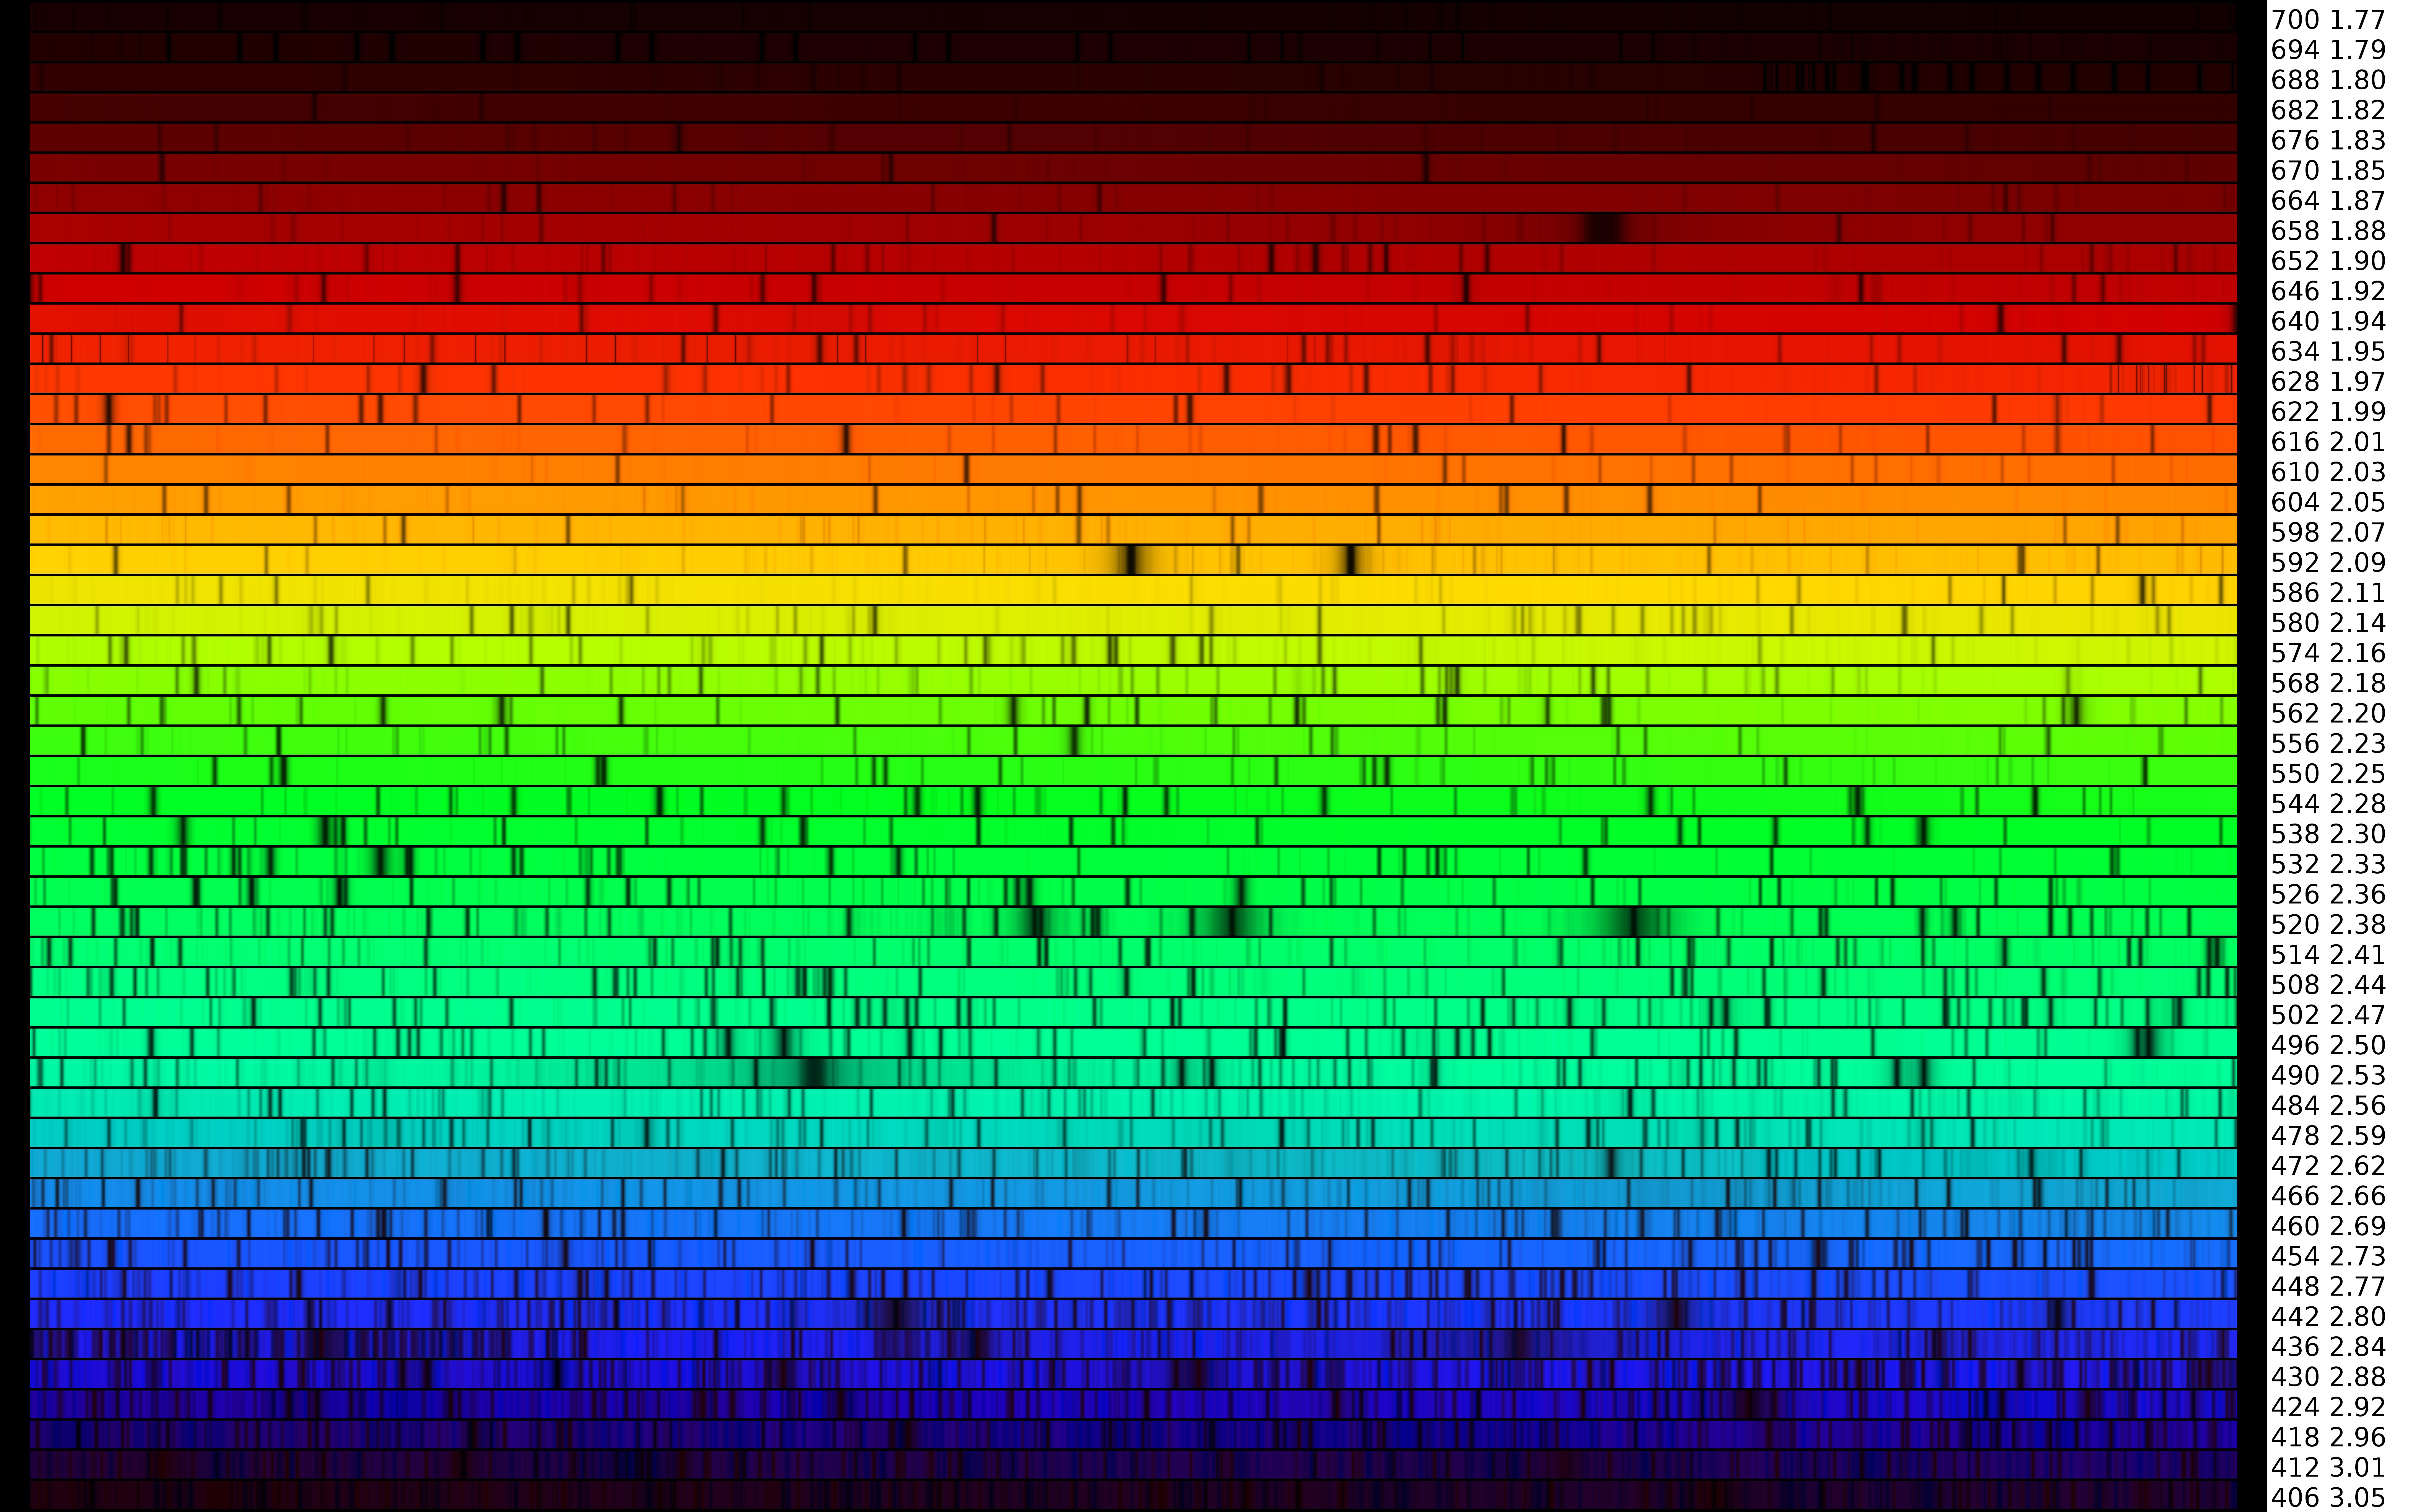
\includegraphics[width=\textwidth]{solarspectrum.jpg}\EC
}

\frame{\frametitle{\textbf{Announcements}}
\large
\BI
\item Provisional study guide posted
\item May be revised on Friday once I see how far we get Thursday
\item Short Mastering Astronomy assignment posted late today, due Tuesday
\item Will catch up on email tomorrow morning
\EI
}

\frame{\frametitle{\textbf{Exam preparation schedule}}
\BI
\large
\item Clinic hours tonight (4:30-6:30) 
\item Quick answers to study questions all day Wednesday
\item Help session Friday held in room 208 from 9:30-11:30 and in the Clinic from 1:30-3:30
\item Review on Sunday:
\BI
\large
\item \color{A}A: 2:30 PM-5 PM
\item \color{B}B: 8:30 PM-11:30 PM
\EI
\item Extended clinic hours next Monday: 2PM-6PM
\EI
}

\frame{\frametitle{\bf Emission spectra}

Last time we saw that atoms can emit light of particular wavelengths/energies corresponding to their atomic transitions.

\BS

This gives us {\it emission spectra} consisting of bright lines (from NMSU Astronomy):

\BC
\includegraphics[width=0.5\textwidth]{emission-spectra.png}
\EC
}



\frame{\frametitle{\bf Absorption spectra}

\large

Elements can also {\it absorb} wavelengths of these particular wavelengths as well.

\BS

(Remember that these atomic transitions can go both ways.)

\BS

Other colors simply pass through.

\BS

(Molecules have these spectra too: their electron energy levels are more complicated.)

}


\frame{

\BC
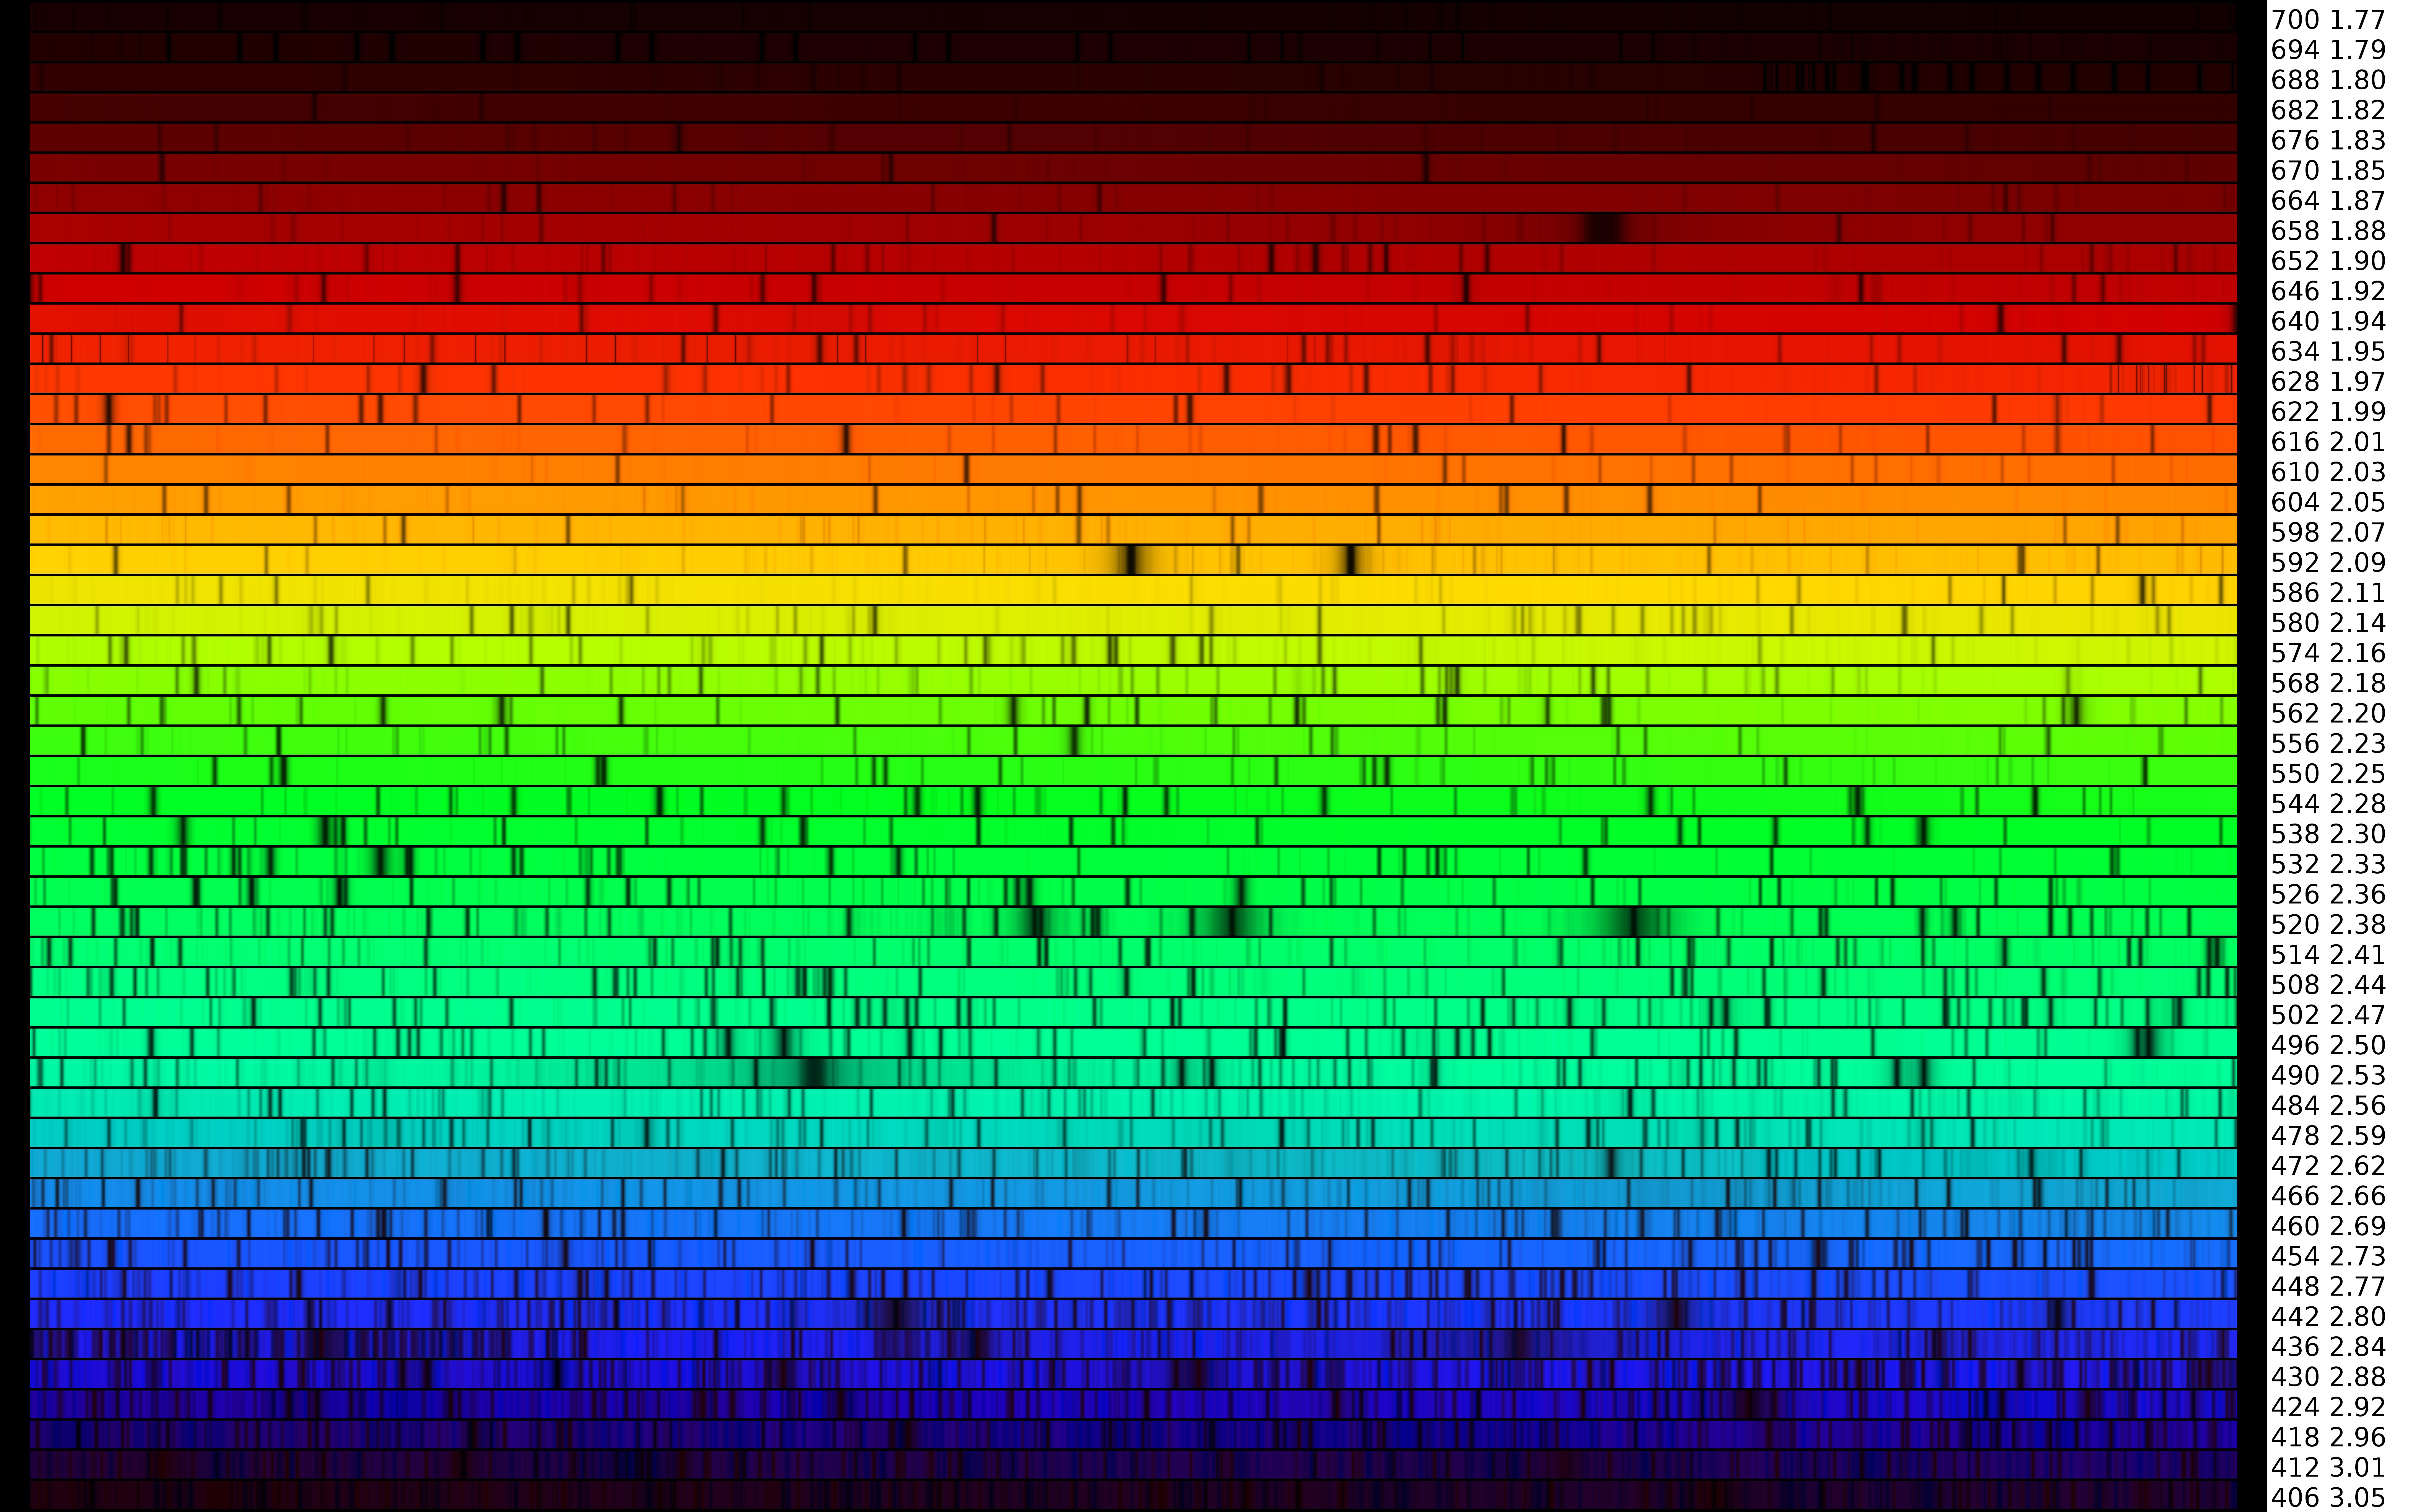
\includegraphics[width=0.7\textwidth]{solarspectrum.jpg}
\EC

\BI
\item The hot core of the Sun emits light of all wavelengths (you'll learn why next class)
\pause
\item The gases in the cooler atmosphere absorb light of their particular wavelengths
\pause
\EI
\BC
\color{Red} \large This picture tells us what's in the Sun!
\EC
}

\frame{

\Large

You discover lines in the solar spectrum that don't correspond to any known element.
What do you conclude?

\BS

\color{A}A: Something about quantum mechanics is different in the Sun\\\BS

\color{B}B: Something about light is different in the Sun\\\BS
\color{C}C: There's an element in the Sun that's not on Earth -- call it {\bf sunium} \\ \BS
\color{D}D: The extreme temperature of the Sun causes new lines to appear in its gas \\ \BS
\pause
\color{E}E: ``Sunium''? There's no such element!
}


\frame{

\BC
\includegraphics[width=0.95\textwidth]{stellar-spectra.jpg}
\BS

\large

All the stars are made of the same stuff -- the same stuff as we are.\pause
\EC
``The cosmos is also within us. We are made of star-stuff. We are a way for the universe to know itself.''

\begin{flushright}--Carl Sagan, {\it Cosmos} \end{flushright}
}

\frame{\frametitle{\textbf What a lucky accident!}
\large 
We're very lucky that atomic transitions happen to lie in our visual range!

There are others that are very interesting to astronomers:

\BI
\item Molecular vibrations: infrared
\pause
\item Molecular {\it rotations}: microwave
\pause
\item ``Hyperfine structure'' energy levels in hydrogen: 21 cm radio waves
\EI

\pause

\normalsize

This last is particularly interesting: it is a very particular frequency, echoing out from
all corners of the Universe, that says: hydrogen is here. (Hydrogen is 75\% of the universe.)
}

\frame{
\BC
\includegraphics[width=0.5\textwidth]{pioneer-10.jpg}
\EC
}

\frame{
\BC
\includegraphics[width=0.8\textwidth]{pioneer-plaque.jpg}
\EC
}

\frame{
\BC
\includegraphics[width=0.7\textwidth]{pioneer-plaque-2.jpg}\\
\includegraphics[width=0.3\textwidth]{hyperfine.jpg}
\EC
}

\frame{
\BC
\Large
If Nature has a ruler, its markings are 21 cm apart.

\pause\BS\BS

\normalsize (TRF people: it's the 60Hz-hum of the universe. :) )
\EC
}

\frame{
\BC
Let's look at that solar spectrum again:

\BS
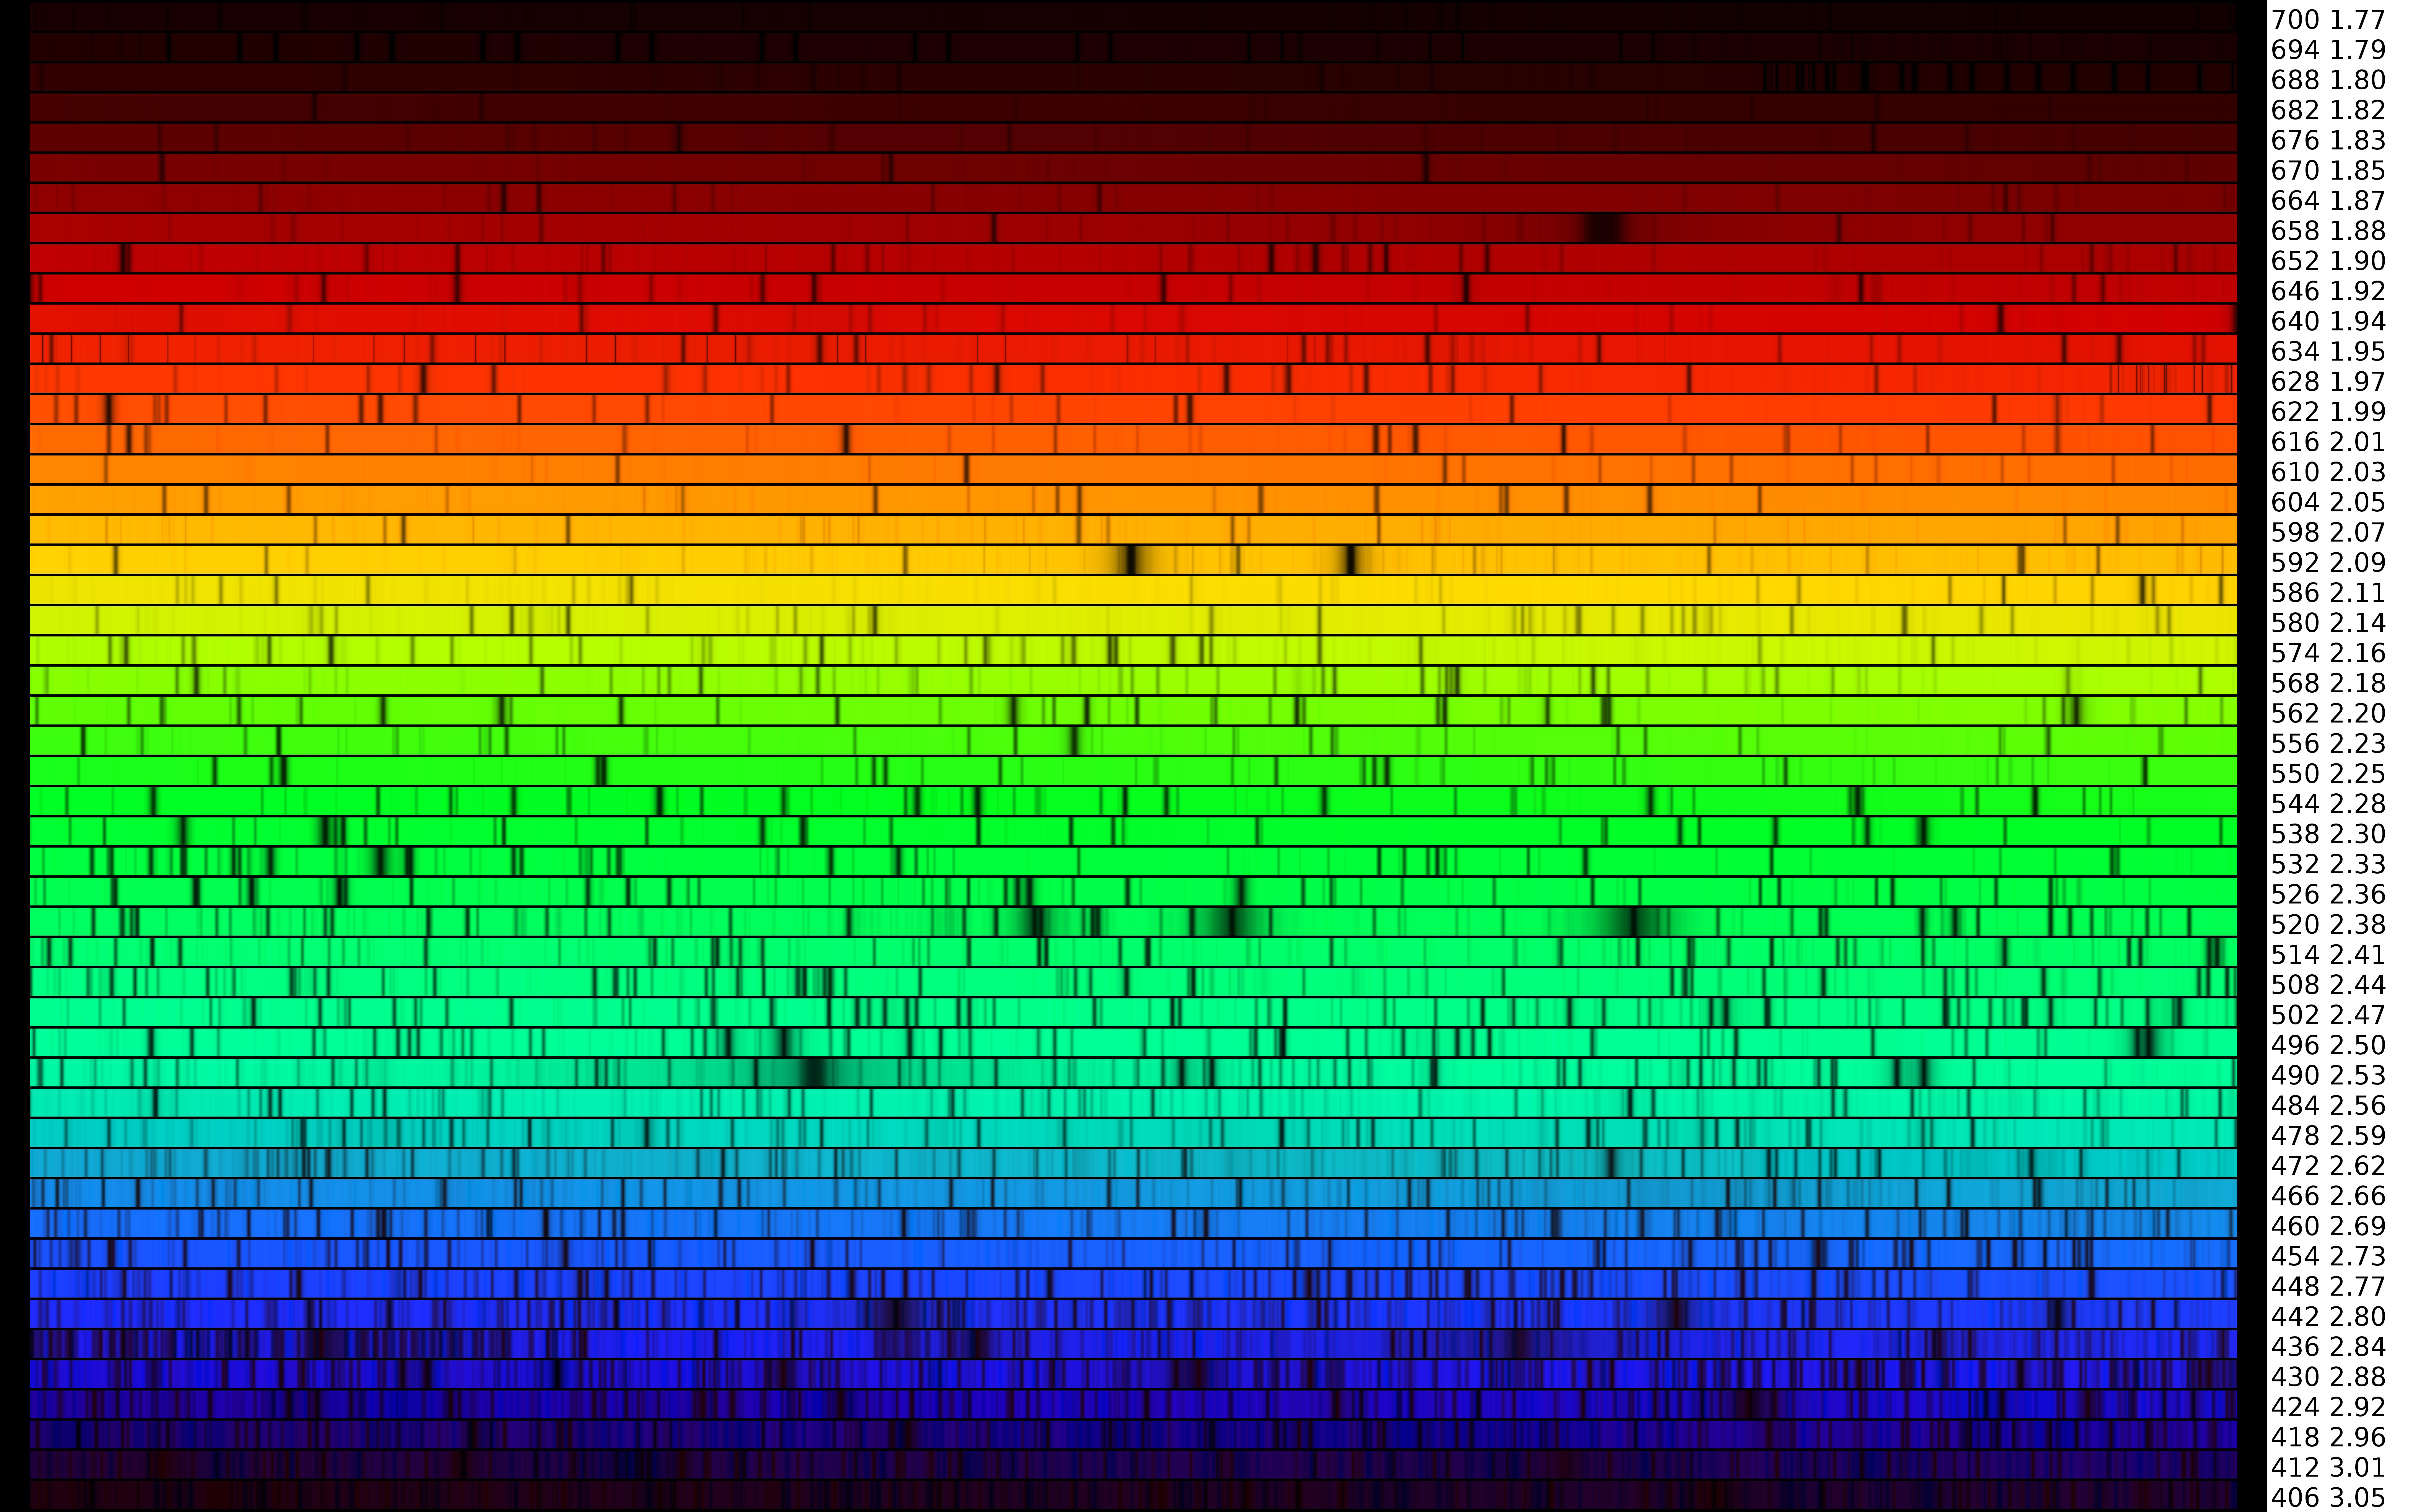
\includegraphics[width=0.7\textwidth]{solarspectrum.jpg}
\EC
\BS

We understand why the dark lines are where they are. But where does that continuous spectrum -- light of {\it all} wavelengths -- come from
in the first place?
}

\frame{\frametitle{\textbf{Thermal radiation}}

\BC
\Large
Objects glow because they're hot.
\EC
\BS
\BS

\BI
\item Any object with a temperature emits electromagnetic radiation (``light'').
\item For objects as warm as we are, this is in the ``far infrared''.
\item As objects heat up, the peak wavelength decreases (the average photon energy increases)
\item As objects heat up, the total intensity emitted goes up {\it rapidly} (proportional to $T^4$)
\item This is also called ``blackbody radiation'' (since even a black object glows if it's warmed up)
\EI

\BS
\BC
See the simulation to see how this works...
\EC
}

\frame{\frametitle{\textbf{Done!}}

\BC
\Large
This is all the physics you need to know.

\BS
\BS
Complete {\it Lecture Tutorials} pp. 59-61 (skip 62).

\pause

Complete {\it Lecture Tutorials} pp. 63-64.

\pause

Finish up {\it Lecture Tutorials} pp. 65-69.

\EC
}





\end{document}

